% JACoW-style working draft.
% Official JACoW class: v3.01 (2026-03-11).
% Latest-CESR production revision for dataset-generation readiness.
\documentclass[letterpaper]{jacow}

\usepackage[english]{babel}
\usepackage{bm}

\begin{document}

\title{HIGH-THROUGHPUT NONLINEAR CLOSED-ORBIT CALCULATION AND RESPONSE-ERROR ANALYSIS IN THE LATEST CESR MODEL BASED ON SciBmad}

% Replace the temporary author metadata before circulation/submission.
\author[1]{J. N. Author}
\affil[1]{Cornell University, Ithaca, NY, USA}

\maketitle

\begin{abstract}
We present a batched RF-on closed-orbit calculation in SciBmad for the latest
validated CESR charged-particle lattice. A nominal GTPSA response initializes
frozen-Jacobian Newton iterations with explicit closure checks and an
automatic-differentiation fallback. A 36001-state amplitude sweep over all,
horizontal, and vertical steering subspaces converges 36000 states; 62 of 63
fallback attempts recover, and every converged state closes below
$10^{-13}$. At the first sampled radius where the all-control mean residual
exceeds \qty{1}{\micro\metre}, $\rho=1.13$, the means are
\qty{1.445}{\micro\metre} in $x$ and \qty{1.153}{\micro\metre} in $y$.
Exact complete-element sourcing over 1177 elements reconstructs the horizontal
and vertical quadratic targets to relative residuals of
$1.309\times10^{-14}$ and $1.312\times10^{-14}$. Normal sextupoles supply
96.508\% and 98.647\% of the corresponding signed projections. A matched
9001-state comparison requires 17.989~s for 16-thread SciBmad physics and
136.797~s for Bmad/Tao configured with 16 OpenMP threads, a 7.605-fold
wall-clock speedup; including reusable-model SciBmad setup requires 22.842~s.
\end{abstract}

\section{Introduction}

Accelerator datasets intended for model calibration, surrogate learning, and
control studies must be more than large and computationally inexpensive: their
labels should represent physically self-consistent states, carry reproducible
solver provenance, and remain accurate over a quantified input domain.
High-speed differentiable simulation makes large-scale generation practical
\cite{kaiser2024,wan2025,huhn2025}, and learned map models show the value of
such data for beam-based error identification \cite{caliari2025}.  For an orbit
dataset, the central label is the closed orbit associated with each sampled
control state.  It should satisfy the six-dimensional RF-on periodic condition,
and the error from replacing that nonlinear solution with a nominal linear
response should be known.

The orbit-response matrix provides an efficient local model, but nonlinear
lattice maps have visible effects with large corrector amplitudes, particularly
through sextupoles. Large-amplitude and off-energy closed-orbit measurements have
therefore been used to characterize and correct nonlinear optics
\cite{olsson2020,huang2024}.  Generating reference data in this regime requires
repeated nonlinear fixed-point solutions.  A useful implementation must combine
throughput with explicit closure tests, robust convergence, and a mapped
relationship between linear-response error and nonlinear-solver survival.

We apply this workflow with SciBmad~\cite{scibmad2026} to the RF-on main branch
of a Bmad-compatible latest CESR model~\cite{sagan2006,cesrModel}: a
\qty{6}{\giga\electronvolt} positron lattice with four
\qty{1.5}{\mega\volt} RF cavities, 103 independently varied normal-steering
controls, and 144 detector locations reporting both transverse planes. The
selected controls comprise 58 horizontal and 45 vertical channels; the
detector vector therefore contains 288 ordered observables. We map response
error and convergence over corrector amplitude and input subspace, then
attribute the quadratic detector target to complete lattice elements. The
calculation does not vary girder pitch or photon branches, so the documented
curved-DQX pitch and general mirror-optics limitations do not enter the
reported observables. The study is synthetic numerical analysis, not a
real-machine validation.

\section{Orbit Calculation Methodology}

The CESR configuration is loaded from
\texttt{latest\_cesr\_scibmad\_repaired.jl} in SciBmad 0.4.1 with RF on and
branch 0. All dimensions and ordered labels are discovered from the runtime
control and detector registries rather than fixed historical constants.

For corrector vector $\bm k$, the RF-on closed orbit $\bm z_*$ satisfies the
six-dimensional fixed-point equation
\begin{equation}
  \bm F(\bm z_*,\bm k)=\mathcal M(\bm z_*,\bm k)-\bm z_*=0 .
  \label{eq:fixedpoint}
\end{equation}
SciBmad evaluates many corrector states as one batch.  A cached
$6\times103$ nominal response supplies the initial value as
$\bm z_{\mathrm{init}}=\bm z_0+R\Delta\bm k$.  Newton iterations then evaluate the nonlinear one-turn residual while reusing one nominal $6\times6$
Jacobian factorization. When a lane does not converge, a sample-specific
automatic-differentiation Jacobian is used as fallback. Every accepted state
is tested against the six-dimensional periodic closure, with relative and
absolute tolerances of $10^{-12}$ and $10^{-13}$.

\section{Latest-CESR Nonlinear Calculation}

For the active correctors $A$ in a selected input subspace, let
$k_{\mathrm{rms}}=\operatorname{rms}(\Delta\bm k_A)$ and define
$\rho=k_{\mathrm{rms}}/\qty{5}{\micro\radian}$.  Each sampled Gaussian
direction $\bm d$ is normalized independently to
$\operatorname{rms}(\bm d_A)=1$, so that
$\Delta\bm k=\rho\bm d\,\cdot \qty{5}{\micro\radian}$. For all-, horizontal-,
and vertical-control inputs, 600 fixed directions are reused at 20 positive
radii from $\rho=0.1$ to 64. Together with one shared nominal reference, this
gives 36001 unique exact states. The five radii retained from the earlier
matched table, $\rho=1.13$, 3.2, 4.53, 6.4, and 9.05, contribute 9000 nonzero
states and are all complete in the latest-ring run.

Table~\ref{tab:nonlinear-calculation} summarizes the matched latest-ring
calculation.
One all-control lane at $\rho=51.2$ does not converge; all other sampled cells,
including $\rho=64$, are complete. This isolated non-monotonic failure is
reported as solver-survival evidence, not as a physical aperture boundary.
For the matched 9001-state comparison, both codes return all states. SciBmad
uses no fallback, requires at most seven iterations, and has maximum closure
$9.992\times10^{-11}$. Tao uses one persistent process configured with 16
OpenMP threads and evaluates the input states sequentially.

\begin{table}[!htb]
  \centering
  \caption{Latest-CESR matched nonlinear closed-orbit calculation.}
  \footnotesize
  \begin{tabular}{@{}lrrr@{}}
    \toprule
    \textbf{Calculation} & \textbf{States} & \textbf{Time [s]} &
    \textbf{Rate [$\mathrm{s}^{-1}$]} \\
    \midrule
    Bmad/Tao (16 thr.) & 9000 & 136.797 & 65.791 \\
    SciBmad physics (16 thr.) & 9000 & 17.989 & 500.318 \\
    SciBmad incl. setup & 9000 & 22.842 & 394.018 \\
    \bottomrule
  \end{tabular}
  \label{tab:nonlinear-calculation}
\end{table}

\section{Orbit Response Error Analysis}
\subsection{General amplitude dependence}
For detector-orbit vector $\bm u$, we can expand about the nominal corrector state input,
\begin{equation}
 \bm u(\Delta\bm k)=\bm u_0+J\Delta\bm k
 +\frac12H[\Delta\bm k,\Delta\bm k]
 +\frac16T[\Delta\bm k,\Delta\bm k,\Delta\bm k]+\cdots .
 \label{eq:taylor}
\end{equation}

The nominal linear-response residual is
$\bm e=\bm u(\Delta\bm k)-\bm u_0-J\Delta\bm k$.  The general sweep uses the
same 600 directions at 20 radii from $\rho=0.1$ to 64 in each input subspace,
which is 36001 nonlinear states in total including the nominal reference.  Detector rms
residuals are summarized by the mean and largest sampled direction at each
radius in Fig.~\ref{fig:general-response-error}.

At $\rho=1.13$, the all-control mean residuals are
\qty{1.445}{\micro\metre} in $x$ and \qty{1.153}{\micro\metre} in $y$.
Vertical-only inputs produce \qty{1.053}{\micro\metre} in $x$ but only
\qty{0.008259}{\micro\metre} in $y$; horizontal-only inputs produce
\qty{0.7308}{\micro\metre} in $x$ and a $y$ residual below
$2\times10^{-13}\,\mu\mathrm m$. Thus $\rho=1.13$ is the first sampled
all-control radius at which the mean in either output plane exceeds an
illustrative \qty{1}{\micro\metre} label-error budget. This is a discrete
sampled crossing, not an interpolated machine limit.

The principal-plane channels remain approximately quadratic through the
moderate-amplitude range. The much smaller vertical-only $y$ residual grows
approximately cubically over the five tabulated radii, while the
horizontal-only $y$ channel remains at numerical-zero scale. A dataset must
therefore state its accepted output error and cannot infer one global input
limit from corrector rms alone.

All 600 directions in all three scenarios converge through $\rho=36.2$.
At $\rho=51.2$, 599/600 all-control directions converge; every other sampled
scenario-radius cell is complete. Overall, 36000/36001 states converge, with
62 lanes recovered by fallback and one retained failure whose closure norm is
4.35066.

\begin{figure}[!b]
  \centering
  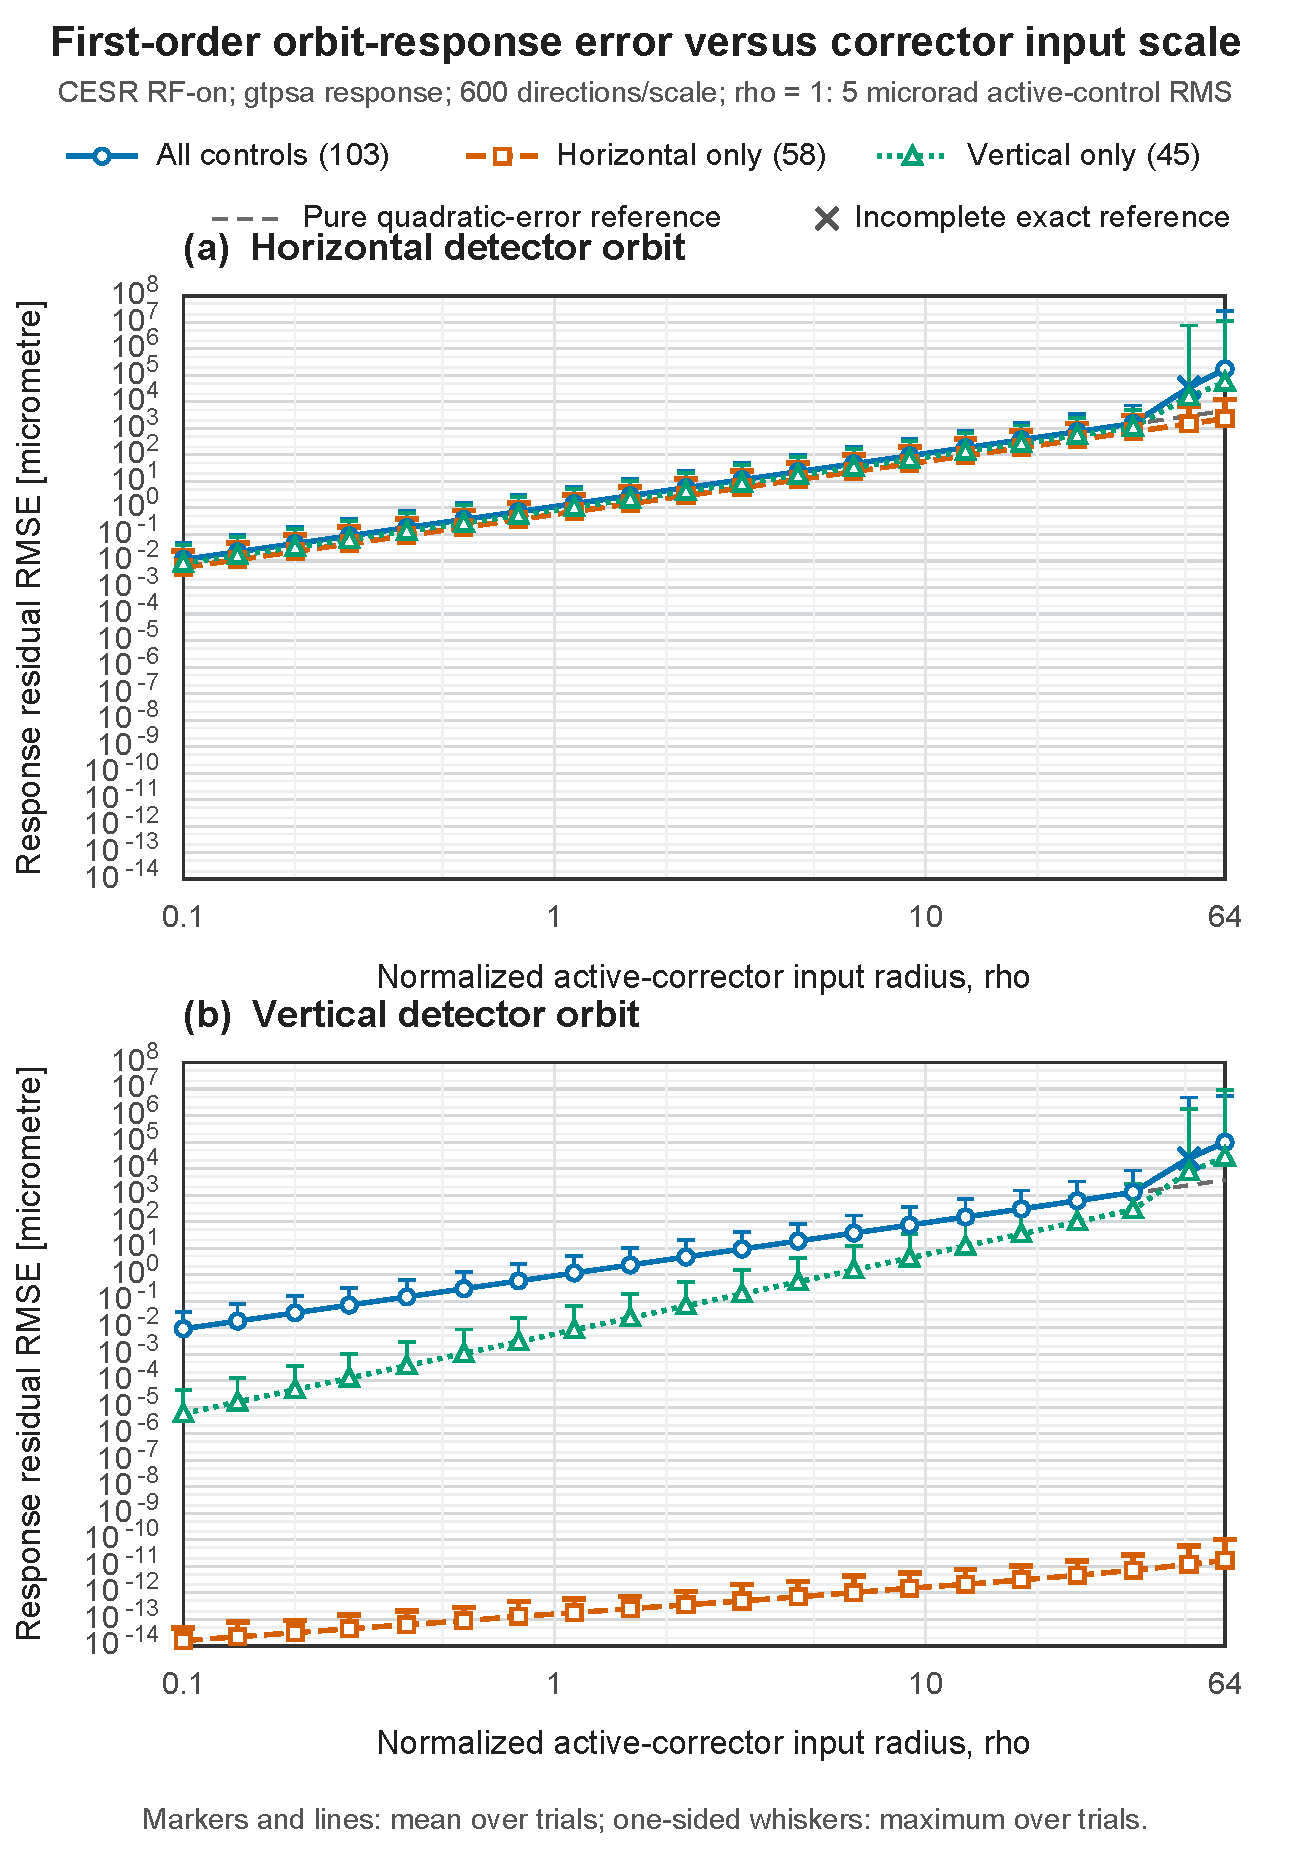
\includegraphics[width=\columnwidth]{figures/scibmad_orbit_response_error_stacked.pdf}
  \caption{Growth of the horizontal and vertical nonlinear orbit-response
  residuals with corrector-input radius over 600 fixed directions per radius.
  Curves show the mean detector rms, whiskers the largest sampled direction,
  and crosses cells with incomplete exact references.}
  \label{fig:general-response-error}
\end{figure}

\begin{figure*}[!t]
  \centering
  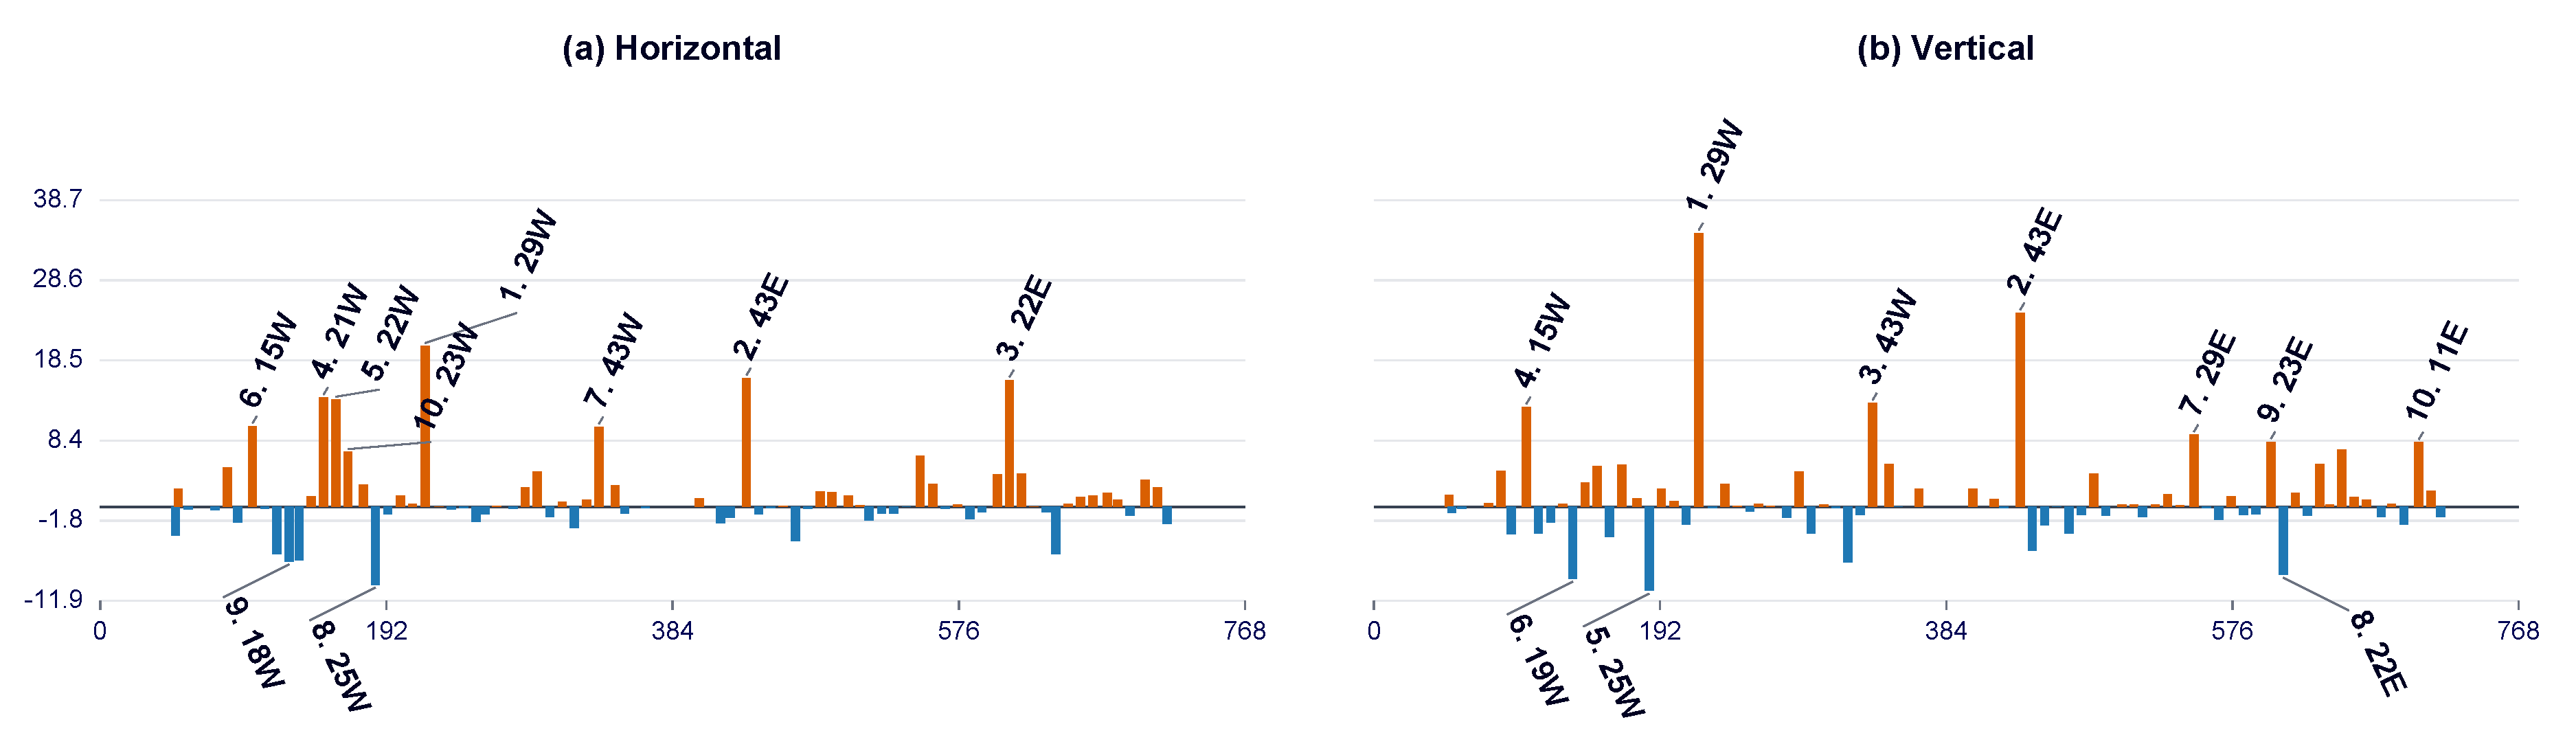
\includegraphics[width=\textwidth]{figures/thick_sextupole_signed_contributions_paired.pdf}
  \caption{Signed complete-element projections of the 76 active normal
  sextupoles onto the all-corrector quadratic detector targets, plotted against
  ring position for (a) horizontal and (b) vertical output.  Labels mark the
  ten largest absolute projections in each plane; positive and negative bars
  display constructive and cancelling contributions to the family sum.}
  \label{fig:sextupole-signed-contributions}
\end{figure*}
\subsection{Second-order lattice-element attribution}

The amplitude sweep identifies the quadratic regime but does not assign its
detector error to lattice elements.  For the 100 corrector-direction pairs
used below, the implicit GTPSA solution supplies the first- and second-order
periodic orbit at every element boundary.  \\
Let $A_j$ be the first-order (orbit) map of
complete element $j$, and let $\bm S_{j,-}^{(d)}$ and $\bm S_{j,+}^{(d)}$ be
the direction-contracted second-order states at its entrance and exit.  The
new local source generated by that element will then be
\begin{equation}
 \bm g_j^{(d)}=\bm S_{j,+}^{(d)}-A_j\bm S_{j,-}^{(d)}.
 \label{eq:complete-element-source}
\end{equation}
Each source is propagated through the periodic ring to all
144 detectors. For output plane $p\in\{x,y\}$, let $\bm Q_p^{(d)}$ denote the
all-corrector direction-contracted quadratic target.
Summing propagated vectors from all 1177 elements reconstructs
$\bm Q_x^{(d)}$ and $\bm Q_y^{(d)}$, giving ensemble relative residuals
$1.309\times10^{-14}$ and $1.312\times10^{-14}$, respectively.

For family $F$, let $\bm C_{F,p}^{(d)}$ denote its summed propagated detector
vector.  Then we can calculate both the ensemble signed projection and magnitude ratio
\begin{equation}
 \eta_{F,p}=\frac{\sum_d\bm C_{F,p}^{(d)}\mathbin{\cdot}\bm Q_p^{(d)}}
 {\sum_d\|\bm Q_p^{(d)}\|^2},\qquad
 \mu_{F,p}=\left(\frac{\sum_d\|\bm C_{F,p}^{(d)}\|^2}
 {\sum_d\|\bm Q_p^{(d)}\|^2}\right)^{1/2}.
 \label{eq:family-attribution}
\end{equation}

For either output plane the $\eta_{F,p}$ values add to unity; the
$\mu_{F,p}$ values would not as the vectors have different directions.
The complete 10-family partition is shown in
Table~\ref{tab:element-families}. Normal sextupoles supply 96.508\% of the
horizontal and 98.647\% of the vertical signed projection. Sector bends and
drift/geometric maps are the leading secondary families. Kicker and
quadrupole sources remain visible below the percent level, while wiggler and
RF sources are negligible for these observables. Coupling, fringe, and
kinematic effects remain inside the complete-element maps.

\begin{table}[!t]
  \centering
  \scriptsize
  \setlength{\tabcolsep}{2.2pt}
  \begin{tabular}{@{}lrrrrr@{}}
    \toprule
    & & \multicolumn{2}{c}{Horizontal $\bm Q_x$}
        & \multicolumn{2}{c}{Vertical $\bm Q_y$} \\
    \cmidrule(lr){3-4}\cmidrule(l){5-6}
    \textbf{Family} & \textbf{N}
      & $\eta_{F,x}$ [\%] & $\mu_{F,x}$ [\%]
      & $\eta_{F,y}$ [\%] & $\mu_{F,y}$ [\%] \\
    \midrule
    Normal sextupole & 76  & +96.508 & 99.295 & +98.647 & 99.859 \\
    Sector bend      & 98  &  +1.702 & 11.993 &  +0.384 &  6.833 \\
    Drift/geometric  & 562 &  +1.008 &  6.843 &  +0.502 &  5.128 \\
    Kicker           & 82  &  +0.395 &  2.480 &  +0.246 &  1.966 \\
    Quadrupole       & 122 &  +0.357 &  2.349 &  +0.203 &  1.830 \\
    RF cavity        & 4   &  +0.021 &  0.146 &  +0.017 &  0.135 \\
    Wiggler          & 3   &  +0.005 &  0.067 &  +0.001 &  0.074 \\
    Octupole         & 2   &  +0.003 &  0.028 &  -0.000 &  0.025 \\
    Other sextupole  & 6   &  +0.002 &  0.015 &  +0.000 &  0.009 \\
    Marker           & 222 &  +0.000 &  0.000 &  -0.000 &  0.000 \\
    \bottomrule
  \end{tabular}
  \caption{Complete-element family attribution of the horizontal and vertical
  all-corrector quadratic targets.  Signed projections $\eta_{F,p}$ are
  additive; magnitude ratios $\mu_{F,p}$ are not.}
  \label{tab:element-families}
\end{table}

The complete normal-sextupole vectors leave relative residuals of 23.618\%
for $x$ and 15.569\% for $y$, whereas the all-element reconstruction retains
the near-machine-precision closure quoted above.  The sextupole family is
therefore the dominant projected source but not a closed decomposition by
itself; the remaining complete-element families and their interference must
be retained when reconstructing the detector vector.

Figure~\ref{fig:sextupole-signed-contributions} resolves the normal-sextupole
family into its 76 signed element projections around the \qty{768.438}{\metre}
ring. The positive and negative bars show that the family result is a signed,
phase-dependent sum rather than a collection of positive error shares.



\subsection{Direction dependence and physical interpretation}

Normal-sextupole dominance is robust across the fixed direction ensemble, but
individual directions exhibit substantial constructive and cancelling
interference. Table~\ref{tab:direction-statistics} gives the P10,
median, and P90 direction-resolved family statistics. The median signed
projections are 96.590\% in $x$ and 99.775\% in $y$; the P90 signed values
exceed 100\%, which is allowed because the remaining family vectors cancel
part of the normal-sextupole vector.

This behavior is consistent with the ordinary normal-sextupole local source
and periodic closed-orbit transport picture \cite{wolski2013,lamont2020}, but
the present exact attribution does not reduce the complete coupled transport
to an uncoupled thin-lens predictor. A direction-matched source--beta--phase
correlation study has not yet been rerun in production on the latest lattice;
historical-ring correlations are therefore not used as latest-CESR evidence.

\begin{table}[!htb]
  \centering
  \caption{Direction-resolved normal-sextupole family statistics [\%].}
  \scriptsize
  \setlength{\tabcolsep}{3.3pt}
  \begin{tabular}{@{}lrrrr@{}}
    \toprule
    \textbf{Statistic} & $\eta_{F,x}$ & $\mu_{F,x}$ & $\eta_{F,y}$ & $\mu_{F,y}$ \\
    \midrule
    P10    & 90.452 & 95.236 & 89.809 & 92.310 \\
    Median & 96.590 & 99.178 & 99.775 & 99.875 \\
    P90    & 101.268 & 103.487 & 108.184 & 110.876 \\
    \bottomrule
  \end{tabular}
  \label{tab:direction-statistics}
\end{table}

\section{Conclusion}

Batched latest-CESR SciBmad calculations converged for 36000 of 36001 sampled
RF-on states, including 62 recovered fallback lanes, with accepted closure
below $10^{-13}$. The amplitude sweep confirms that linear-response error
depends strongly on both corrector subspace and detector channel, so a single
corrector-rms limit is insufficient for dataset sampling. Exact sourcing over
all 1177 elements closes both quadratic detector targets near machine
precision and identifies the 76 active normal sextupoles as the leading signed
source, at 96.508\% in $x$ and 98.647\% in $y$. These latest-lattice results
support nonlinear label generation with explicit closure, fallback, and
channel-aware sampling metadata. The matched 9001-state calculation gives a
7.605-fold SciBmad physics-time wall-clock speedup over 16-thread native
Bmad/Tao; including reusable-model SciBmad setup, the speedup is 5.989-fold.

% IPAC contributed papers may place references on a fourth page.
\clearpage

\begin{thebibliography}{99}

  \bibitem{kaiser2024}
    J. Kaiser, C. Xu, A. Eichler, and A. Santamaria Garcia,
    ``Bridging the gap between machine learning and particle accelerator
    physics with high-speed, differentiable simulations'',
    \textit{Phys. Rev. Accel. Beams}, vol.~27, p.~054601, 2024.
    \doi{10.1103/PhysRevAccelBeams.27.054601}

  \bibitem{wan2025}
    J. Wan, H. Alamprese, C. Ratcliff, J. Qiang, and Y. Hao,
    ``JuTrack: A Julia package for auto-differentiable accelerator modeling
    and particle tracking'', \textit{Comput. Phys. Commun.}, vol.~309,
    p.~109497, 2025. \doi{10.1016/j.cpc.2024.109497}

  \bibitem{huhn2025}
    F. Huhn and F. M. Velotti, ``Differentiable simulations for particle
    tracking in accelerators: Analysis, benchmarking, and optimization'',
    \textit{Phys. Rev. Accel. Beams}, vol.~28, p.~114603, 2025.
    \doi{10.1103/cbds-lst1}

  \bibitem{caliari2025}
    C. Caliari, A. Oeftiger, and O. Boine-Frankenheim,
    ``Beam-based identification of magnetic field errors in a synchrotron
    using deep Lie map networks'', \textit{Phys. Rev. Accel. Beams}, vol.~28,
    p.~024601, 2025. \doi{10.1103/PhysRevAccelBeams.28.024601}

  \bibitem{olsson2020}
    D. K. Olsson, A. Andersson, and M. Sj\"ostr\"om,
    ``Nonlinear optics from off-energy closed orbits'',
    \textit{Phys. Rev. Accel. Beams}, vol.~23, p.~102803, 2020.
    \doi{10.1103/PhysRevAccelBeams.23.102803}

  \bibitem{huang2024}
    X. Huang, ``Correction of nonlinear lattice with closed orbit
    modulation'', in \textit{Proc. IPAC'24}, Nashville, TN, USA, May 2024,
    pp.~3056--3059. \doi{10.18429/JACoW-IPAC2024-THPC32}

  \bibitem{sagan2006}
    D. Sagan, ``Bmad: A relativistic charged particle simulation library'',
    \textit{Nucl. Instrum. Methods Phys. Res. A}, vol.~558, pp.~356--359,
    2006. \doi{10.1016/j.nima.2005.11.001}

  \bibitem{scibmad2026}
    M. G. Signorelli \textit{et al.}, ``SciBmad: A differentiable,
    GPU-parallelized software library for particle accelerator design,
    nonlinear analysis, and machine learning'', presented at IPAC'26,
    Deauville, France, May 2026, paper THP5325.

  \bibitem{cesrModel}
    J. N. Author, ``CESR digital twin in SciBmad'', GitHub repository, 2026.
    \url{https://github.com/6teamFurina/CESR-Project}

  \bibitem{wolski2013}
    A. Wolski and D. Newton, ``Coupling and alignment'', in
    \textit{Design of Electron Storage and Damping Rings}, U.S. Particle
    Accelerator School, Fort Collins, CO, USA, Jun. 2013, Lecture~5.
    \url{https://uspas.fnal.gov/materials/13CSU/Lecture5.pdf}

  \bibitem{lamont2020}
    M. Lamont \textit{et al.}, ``Accelerator operations'', in
    \textit{Particle Physics Reference Library}, S. Myers and H. Schopper,
    Eds. Cham, Switzerland: Springer, 2020, pp.~519--583.
    \doi{10.1007/978-3-030-34245-6_9}

\end{thebibliography}

\end{document}
